% In your document preamble: \usepackage{booktabs}, \usepackage{hyperref}, \usepackage{longtable}, \usepackage{caption}
\scriptsize
\setlength{\tabcolsep}{3pt}
\begin{longtable}{llllrr@{\hspace{0.8cm}}llllrr}
\captionsetup{labelformat=empty}
\caption{\textbf{SI Table S7. Data for BET-ET Domain Receptors}}
\label{tab:st7} \\
\toprule
apo\_pdb & holo\_pdb & apo\_bmrb & holo\_bmrb & F1 & MCC & apo\_pdb & holo\_pdb & apo\_bmrb & holo\_bmrb & F1 & MCC \\
\midrule
\endfirsthead
\caption[]{(continued)} \\
\toprule
apo\_pdb & holo\_pdb & apo\_bmrb & holo\_bmrb & F1 & MCC & apo\_pdb & holo\_pdb & apo\_bmrb & holo\_bmrb & F1 & MCC \\
\midrule
\endhead
\bottomrule
\endfoot
\bottomrule
\endlastfoot
\href{https://www.rcsb.org/structure/7JMY}{7JMY} & \href{https://www.rcsb.org/structure/7JYN}{7JYN} & \href{https://bmrb.io/data_library/summary/index.php?bmrbId=30782}{30782} & \href{https://bmrb.io/data_library/summary/index.php?bmrbId=30790}{30790} & 0.53 & 0.43 & \href{https://www.rcsb.org/structure/2JNS}{2JNS} & \href{https://www.rcsb.org/structure/2NCZ}{2NCZ} & \href{https://bmrb.io/data_library/summary/index.php?bmrbId=15125}{15125} & \href{https://bmrb.io/data_library/summary/index.php?bmrbId=26041}{26041} & 0.40 & 0.25 \\
\href{https://www.rcsb.org/structure/7JMY}{7JMY} & \href{https://www.rcsb.org/structure/7JYZ}{7JYZ} & \href{https://bmrb.io/data_library/summary/index.php?bmrbId=30782}{30782} & \href{https://bmrb.io/data_library/summary/index.php?bmrbId=30791}{30791} & 0.50 & 0.40 & \href{https://www.rcsb.org/structure/2JNS}{2JNS} & \href{https://www.rcsb.org/structure/2ND0}{2ND0} & \href{https://bmrb.io/data_library/summary/index.php?bmrbId=15125}{15125} & \href{https://bmrb.io/data_library/summary/index.php?bmrbId=26042}{26042} & 0.31 & 0.09 \\
\href{https://www.rcsb.org/structure/7JMY}{7JMY} & \href{https://www.rcsb.org/structure/7JQ8}{7JQ8} & \href{https://bmrb.io/data_library/summary/index.php?bmrbId=30782}{30782} & \href{https://bmrb.io/data_library/summary/index.php?bmrbId=30786}{30786} & 0.51 & 0.37 & \href{https://www.rcsb.org/structure/2JNS}{2JNS} & \href{https://www.rcsb.org/structure/2ND1}{2ND1} & \href{https://bmrb.io/data_library/summary/index.php?bmrbId=15125}{15125} & \href{https://bmrb.io/data_library/summary/index.php?bmrbId=26043}{26043} & 0.23 & -0.06 \\
\href{https://www.rcsb.org/structure/2JNS}{2JNS} & \href{https://www.rcsb.org/structure/6BNH}{6BNH} & \href{https://bmrb.io/data_library/summary/index.php?bmrbId=15125}{15125} & \href{https://bmrb.io/data_library/summary/index.php?bmrbId=30373}{30373} & 0.48 & 0.36 & \href{https://www.rcsb.org/structure/2JNS}{2JNS} & \href{https://www.rcsb.org/structure/6BGG}{6BGG} & \href{https://bmrb.io/data_library/summary/index.php?bmrbId=15125}{15125} & \href{https://bmrb.io/data_library/summary/index.php?bmrbId=30367}{30367} & 0.14 & -0.08 \\
\end{longtable}

\begin{figure}[htbp]
\centering
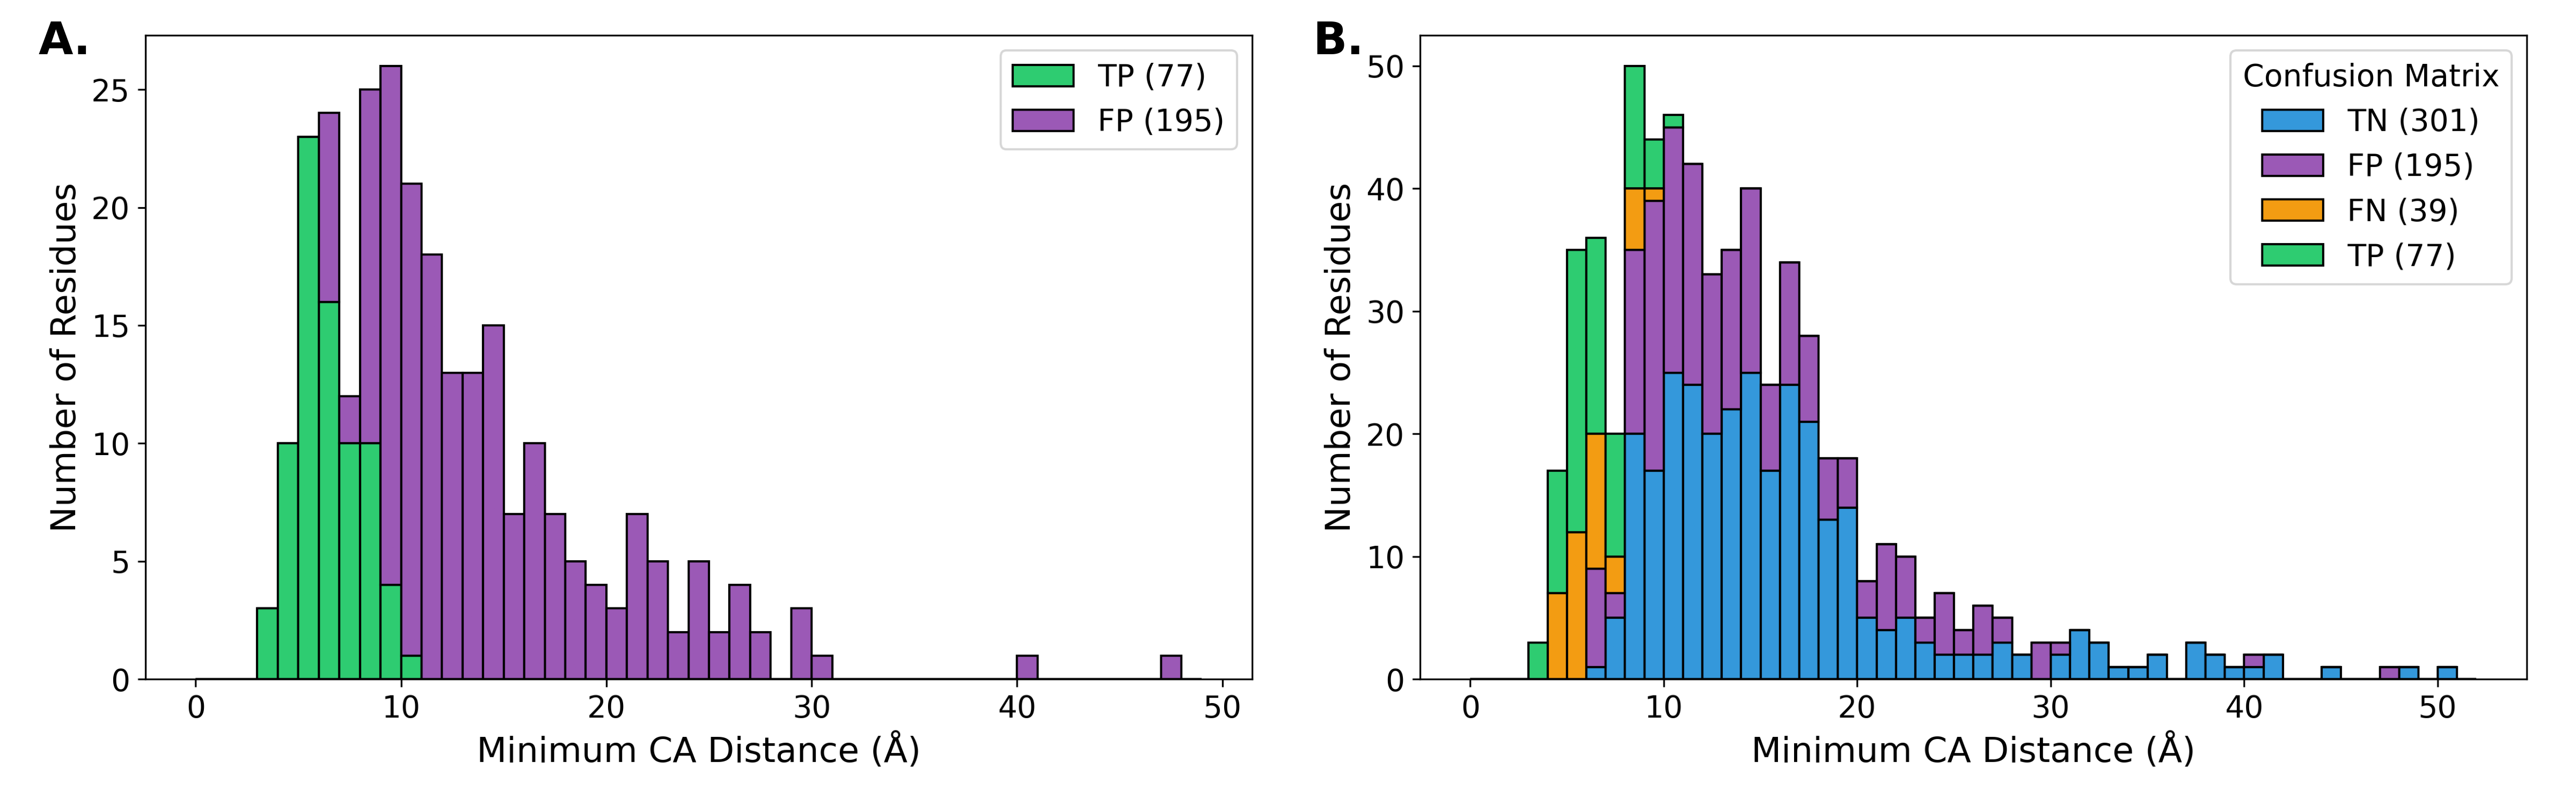
\includegraphics[width=\linewidth]{SF6_BET_ET.png}
\captionsetup{labelformat=empty}
\caption{\textbf{SI Fig. S6. Confusion Matrix Histograms for BET-ET Domain Receptors}}
\label{fig:sf6_bet_et}
\end{figure}
